\documentclass{standalone}
\usepackage{tikz}
\usetikzlibrary{patterns, positioning}


\begin{document}
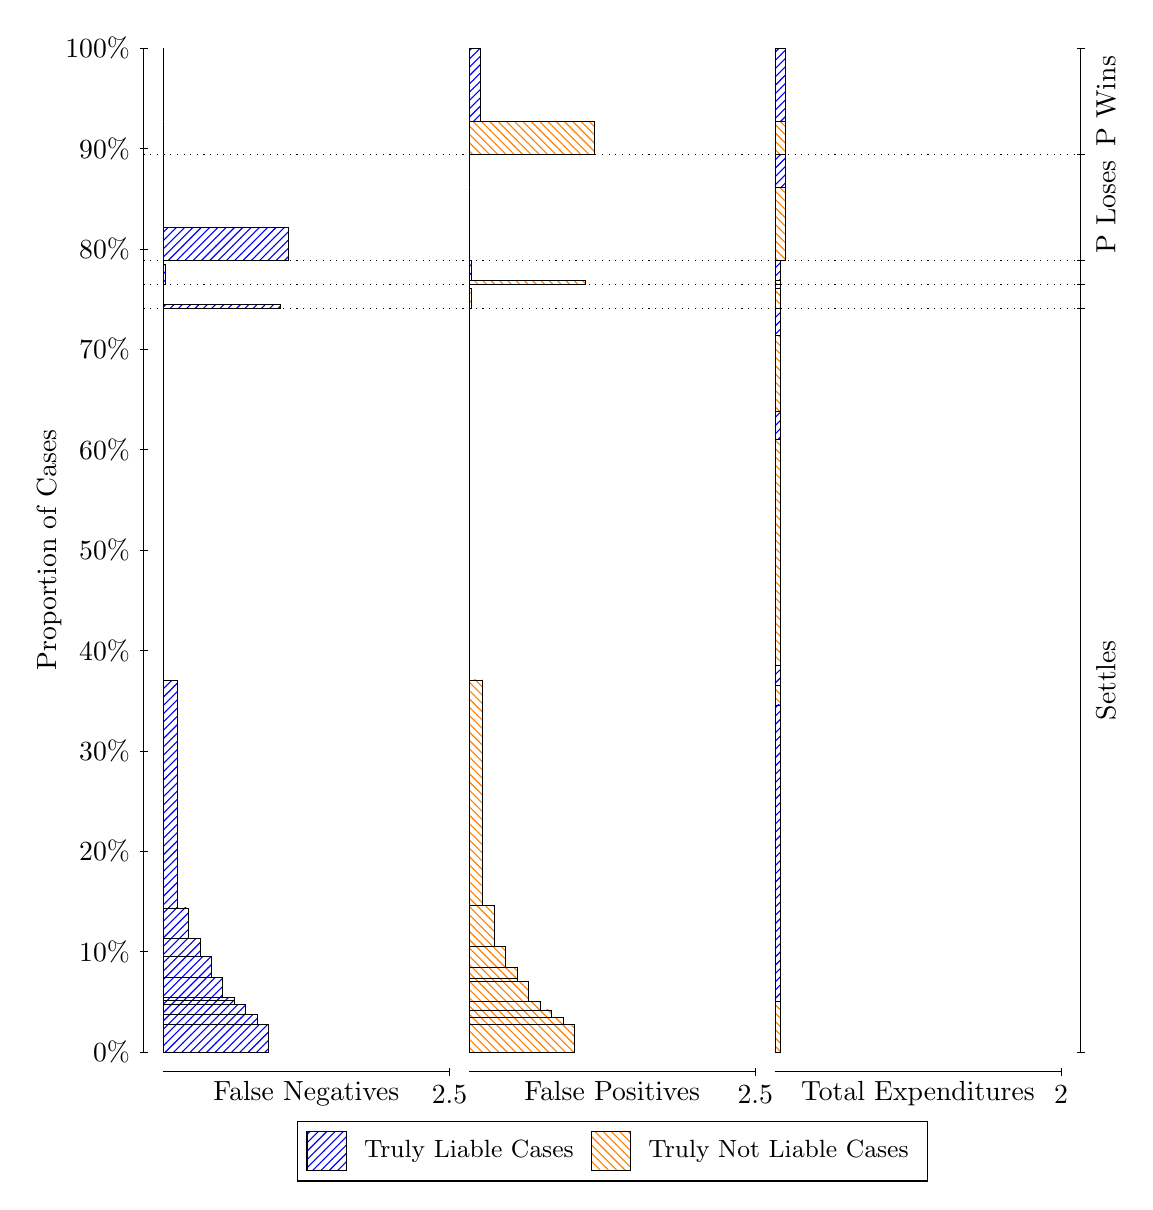
\begin{tikzpicture}
\draw[black, very thin] (1.5,1.75) -- (1.5,14.5);
\node[rotate=90, text=black, anchor=center] at (0.3, 8.125) {Proportion of Cases};
\draw[black, very thin] (1.45,1.75) -- (1.55,1.75);
\node[text=black, anchor=east] at (1.45, 1.75) {0\%};
\draw[black, very thin] (1.45,3.025) -- (1.55,3.025);
\node[text=black, anchor=east] at (1.45, 3.025) {10\%};
\draw[black, very thin] (1.45,4.3) -- (1.55,4.3);
\node[text=black, anchor=east] at (1.45, 4.3) {20\%};
\draw[black, very thin] (1.45,5.575) -- (1.55,5.575);
\node[text=black, anchor=east] at (1.45, 5.575) {30\%};
\draw[black, very thin] (1.45,6.85) -- (1.55,6.85);
\node[text=black, anchor=east] at (1.45, 6.85) {40\%};
\draw[black, very thin] (1.45,8.125) -- (1.55,8.125);
\node[text=black, anchor=east] at (1.45, 8.125) {50\%};
\draw[black, very thin] (1.45,9.4) -- (1.55,9.4);
\node[text=black, anchor=east] at (1.45, 9.4) {60\%};
\draw[black, very thin] (1.45,10.675) -- (1.55,10.675);
\node[text=black, anchor=east] at (1.45, 10.675) {70\%};
\draw[black, very thin] (1.45,11.95) -- (1.55,11.95);
\node[text=black, anchor=east] at (1.45, 11.95) {80\%};
\draw[black, very thin] (1.45,13.225) -- (1.55,13.225);
\node[text=black, anchor=east] at (1.45, 13.225) {90\%};
\draw[black, very thin] (1.45,14.5) -- (1.55,14.5);
\node[text=black, anchor=east] at (1.45, 14.5) {100\%};

\draw[black, very thin] (13.4,1.75) -- (13.4,14.5);
\draw[black, very thin] (13.35,1.75) -- (13.45,1.75);
\node[anchor=west] at (13.35, 1.75) {};
\draw[black, very thin] (13.35,11.191) -- (13.45,11.191);
\node[anchor=west] at (13.35, 11.191) {};
\draw[black, very thin] (13.35,11.497) -- (13.45,11.497);
\node[anchor=west] at (13.35, 11.497) {};
\draw[black, very thin] (13.35,11.805) -- (13.45,11.805);
\node[anchor=west] at (13.35, 11.805) {};
\draw[black, very thin] (13.35,13.149) -- (13.45,13.149);
\node[anchor=west] at (13.35, 13.149) {};
\draw[black, very thin] (13.35,14.5) -- (13.45,14.5);
\node[anchor=west] at (13.35, 14.5) {};

\draw[black, very thin, pattern color=blue, pattern=north east lines] (1.75,1.75) rectangle (3.0852,2.1036);
\draw[black, very thin, pattern color=blue, pattern=north east lines] (1.75,2.1036) rectangle (2.9399,2.2261);
\draw[black, very thin, pattern color=blue, pattern=north east lines] (1.75,2.2261) rectangle (2.7946,2.3545);
\draw[black, very thin, pattern color=blue, pattern=north east lines] (1.75,2.3545) rectangle (2.6492,2.4068);
\draw[black, very thin, pattern color=blue, pattern=north east lines] (1.75,2.4068) rectangle (2.6492,2.4474);
\draw[black, very thin, pattern color=blue, pattern=north east lines] (1.75,2.4474) rectangle (2.5039,2.6999);
\draw[black, very thin, pattern color=blue, pattern=north east lines] (1.75,2.6999) rectangle (2.3586,2.9592);
\draw[black, very thin, pattern color=blue, pattern=north east lines] (1.75,2.9592) rectangle (2.2133,3.1877);
\draw[black, very thin, pattern color=blue, pattern=north east lines] (1.75,3.1877) rectangle (2.0679,3.579);
\draw[black, very thin, pattern color=blue, pattern=north east lines] (1.75,3.579) rectangle (1.9226,6.4647);
\draw[black, very thin, pattern color=orange, pattern=north west lines] (1.75,6.4647) rectangle (1.75,11.191);
\draw[black, very thin, pattern color=blue, pattern=north east lines] (1.75,11.191) rectangle (3.2306,11.241);
\draw[black, very thin, pattern color=orange, pattern=north west lines] (1.75,11.241) rectangle (1.75,11.497);
\draw[black, very thin, pattern color=blue, pattern=north east lines] (1.75,11.497) rectangle (1.7773,11.755);
\draw[black, very thin, pattern color=orange, pattern=north west lines] (1.75,11.755) rectangle (1.75,11.805);
\draw[black, very thin, pattern color=blue, pattern=north east lines] (1.75,11.805) rectangle (3.3396,12.223);
\draw[black, very thin, pattern color=orange, pattern=north west lines] (1.75,12.223) rectangle (1.75,13.149);
\draw[black, very thin, pattern color=orange, pattern=north west lines] (1.75,13.149) rectangle (1.75,13.567);
\draw[black, very thin, pattern color=blue, pattern=north east lines] (1.75,13.567) rectangle (1.75,14.5);
\draw[black, very thin, pattern color=orange, pattern=north west lines] (5.6333,1.75) rectangle (6.9686,2.1034);
\draw[black, very thin, pattern color=orange, pattern=north west lines] (5.6333,2.1034) rectangle (6.8233,2.1914);
\draw[black, very thin, pattern color=orange, pattern=north west lines] (5.6333,2.1914) rectangle (6.6779,2.2838);
\draw[black, very thin, pattern color=orange, pattern=north west lines] (5.6333,2.2838) rectangle (6.5326,2.3931);
\draw[black, very thin, pattern color=orange, pattern=north west lines] (5.6333,2.3931) rectangle (6.3873,2.6431);
\draw[black, very thin, pattern color=orange, pattern=north west lines] (5.6333,2.6431) rectangle (6.2419,2.6856);
\draw[black, very thin, pattern color=orange, pattern=north west lines] (5.6333,2.6856) rectangle (6.2419,2.8226);
\draw[black, very thin, pattern color=orange, pattern=north west lines] (5.6333,2.8226) rectangle (6.0966,3.0952);
\draw[black, very thin, pattern color=orange, pattern=north west lines] (5.6333,3.0952) rectangle (5.9513,3.6068);
\draw[black, very thin, pattern color=orange, pattern=north west lines] (5.6333,3.6068) rectangle (5.8059,6.4761);
\draw[black, very thin, pattern color=blue, pattern=north east lines] (5.6333,6.4761) rectangle (5.6333,11.191);
\draw[black, very thin, pattern color=orange, pattern=north west lines] (5.6333,11.191) rectangle (5.6606,11.447);
\draw[black, very thin, pattern color=blue, pattern=north east lines] (5.6333,11.447) rectangle (5.6333,11.497);
\draw[black, very thin, pattern color=orange, pattern=north west lines] (5.6333,11.497) rectangle (7.1139,11.546);
\draw[black, very thin, pattern color=blue, pattern=north east lines] (5.6333,11.546) rectangle (5.6606,11.805);
\draw[black, very thin, pattern color=orange, pattern=north west lines] (5.6333,11.805) rectangle (5.6333,12.73);
\draw[black, very thin, pattern color=blue, pattern=north east lines] (5.6333,12.73) rectangle (5.6333,13.149);
\draw[black, very thin, pattern color=orange, pattern=north west lines] (5.6333,13.149) rectangle (7.2229,13.567);
\draw[black, very thin, pattern color=blue, pattern=north east lines] (5.6333,13.567) rectangle (5.7696,14.5);
\draw[black, very thin, pattern color=orange, pattern=north west lines] (9.5167,1.75) rectangle (9.5848,2.3931);
\draw[black, very thin, pattern color=blue, pattern=north east lines] (9.5167,2.3931) rectangle (9.5848,6.158);
\draw[black, very thin, pattern color=orange, pattern=north west lines] (9.5167,6.158) rectangle (9.5848,6.4079);
\draw[black, very thin, pattern color=blue, pattern=north east lines] (9.5167,6.4079) rectangle (9.5848,6.6604);
\draw[black, very thin, pattern color=orange, pattern=north west lines] (9.5167,6.6604) rectangle (9.5848,9.5297);
\draw[black, very thin, pattern color=blue, pattern=north east lines] (9.5167,9.5297) rectangle (9.5848,9.8833);
\draw[black, very thin, pattern color=orange, pattern=north west lines] (9.5167,9.8833) rectangle (9.5848,10.847);
\draw[black, very thin, pattern color=blue, pattern=north east lines] (9.5167,10.847) rectangle (9.5848,11.191);
\draw[black, very thin, pattern color=orange, pattern=north west lines] (9.5167,11.191) rectangle (9.5848,11.447);
\draw[black, very thin, pattern color=blue, pattern=north east lines] (9.5167,11.447) rectangle (9.5848,11.497);
\draw[black, very thin, pattern color=orange, pattern=north west lines] (9.5167,11.497) rectangle (9.5848,11.546);
\draw[black, very thin, pattern color=blue, pattern=north east lines] (9.5167,11.546) rectangle (9.5848,11.805);
\draw[black, very thin, pattern color=orange, pattern=north west lines] (9.5167,11.805) rectangle (9.6529,12.73);
\draw[black, very thin, pattern color=blue, pattern=north east lines] (9.5167,12.73) rectangle (9.6529,13.149);
\draw[black, very thin, pattern color=orange, pattern=north west lines] (9.5167,13.149) rectangle (9.6529,13.567);
\draw[black, very thin, pattern color=blue, pattern=north east lines] (9.5167,13.567) rectangle (9.6529,14.5);
\draw[black, dotted] (1.5,11.191) -- (13.4,11.191);
\draw[black, dotted] (1.5,11.497) -- (13.4,11.497);
\draw[black, dotted] (1.5,11.805) -- (13.4,11.805);
\draw[black, dotted] (1.5,13.149) -- (13.4,13.149);
\draw[black, very thin] (1.75,1.5) -- (5.3833,1.5);
\node[text=black, anchor=north] at (3.5667, 1.5) {False Negatives};
\draw[black, very thin] (5.3833,1.45) -- (5.3833,1.55);
\node[text=black, anchor=north] at (5.3833, 1.45) {2.5};

\draw[black, very thin] (5.6333,1.5) -- (9.2667,1.5);
\node[text=black, anchor=north] at (7.45, 1.5) {False Positives};
\draw[black, very thin] (9.2667,1.45) -- (9.2667,1.55);
\node[text=black, anchor=north] at (9.2667, 1.45) {2.5};

\draw[black, very thin] (9.5167,1.5) -- (13.15,1.5);
\node[text=black, anchor=north] at (11.333, 1.5) {Total Expenditures};
\draw[black, very thin] (13.15,1.45) -- (13.15,1.55);
\node[text=black, anchor=north] at (13.15, 1.45) {2};

\node[text=black, centered, rotate=90] at (13.72, 6.4704) {Settles};


\node[text=black, centered, rotate=90] at (13.72, 12.477) {P Loses};
\node[text=black, centered, rotate=90] at (13.72, 13.824) {P Wins};

\draw (7.449999999999999,1.5) node[draw=none] (baseCoordinate) {};
\begin{scope}[align=center]
        \matrix[scale=0.5, draw=black, below=0.5cm of baseCoordinate, nodes={draw}, column sep=0.1cm]{
            \node[rectangle, draw, minimum width=0.5cm, minimum height=0.5cm, pattern color=blue, pattern=north east lines] {}; &
            \node[draw=none, font=\small, text=black] (B) {Truly Liable Cases}; &
            \node[rectangle, draw, minimum width=0.5cm, minimum height=0.5cm, pattern color=orange, pattern=north west lines] {}; &
            \node[draw=none, font=\small, text=black] (B) {Truly Not Liable Cases}; \\
            };
\end{scope}

\end{tikzpicture}
\end{document}